\documentclass{standalone}

\usepackage{tikz}
\usepackage{amsmath}
\usetikzlibrary{arrows}


\begin{document}
\begin{tikzpicture}[>=latex]
	% Ebene
	%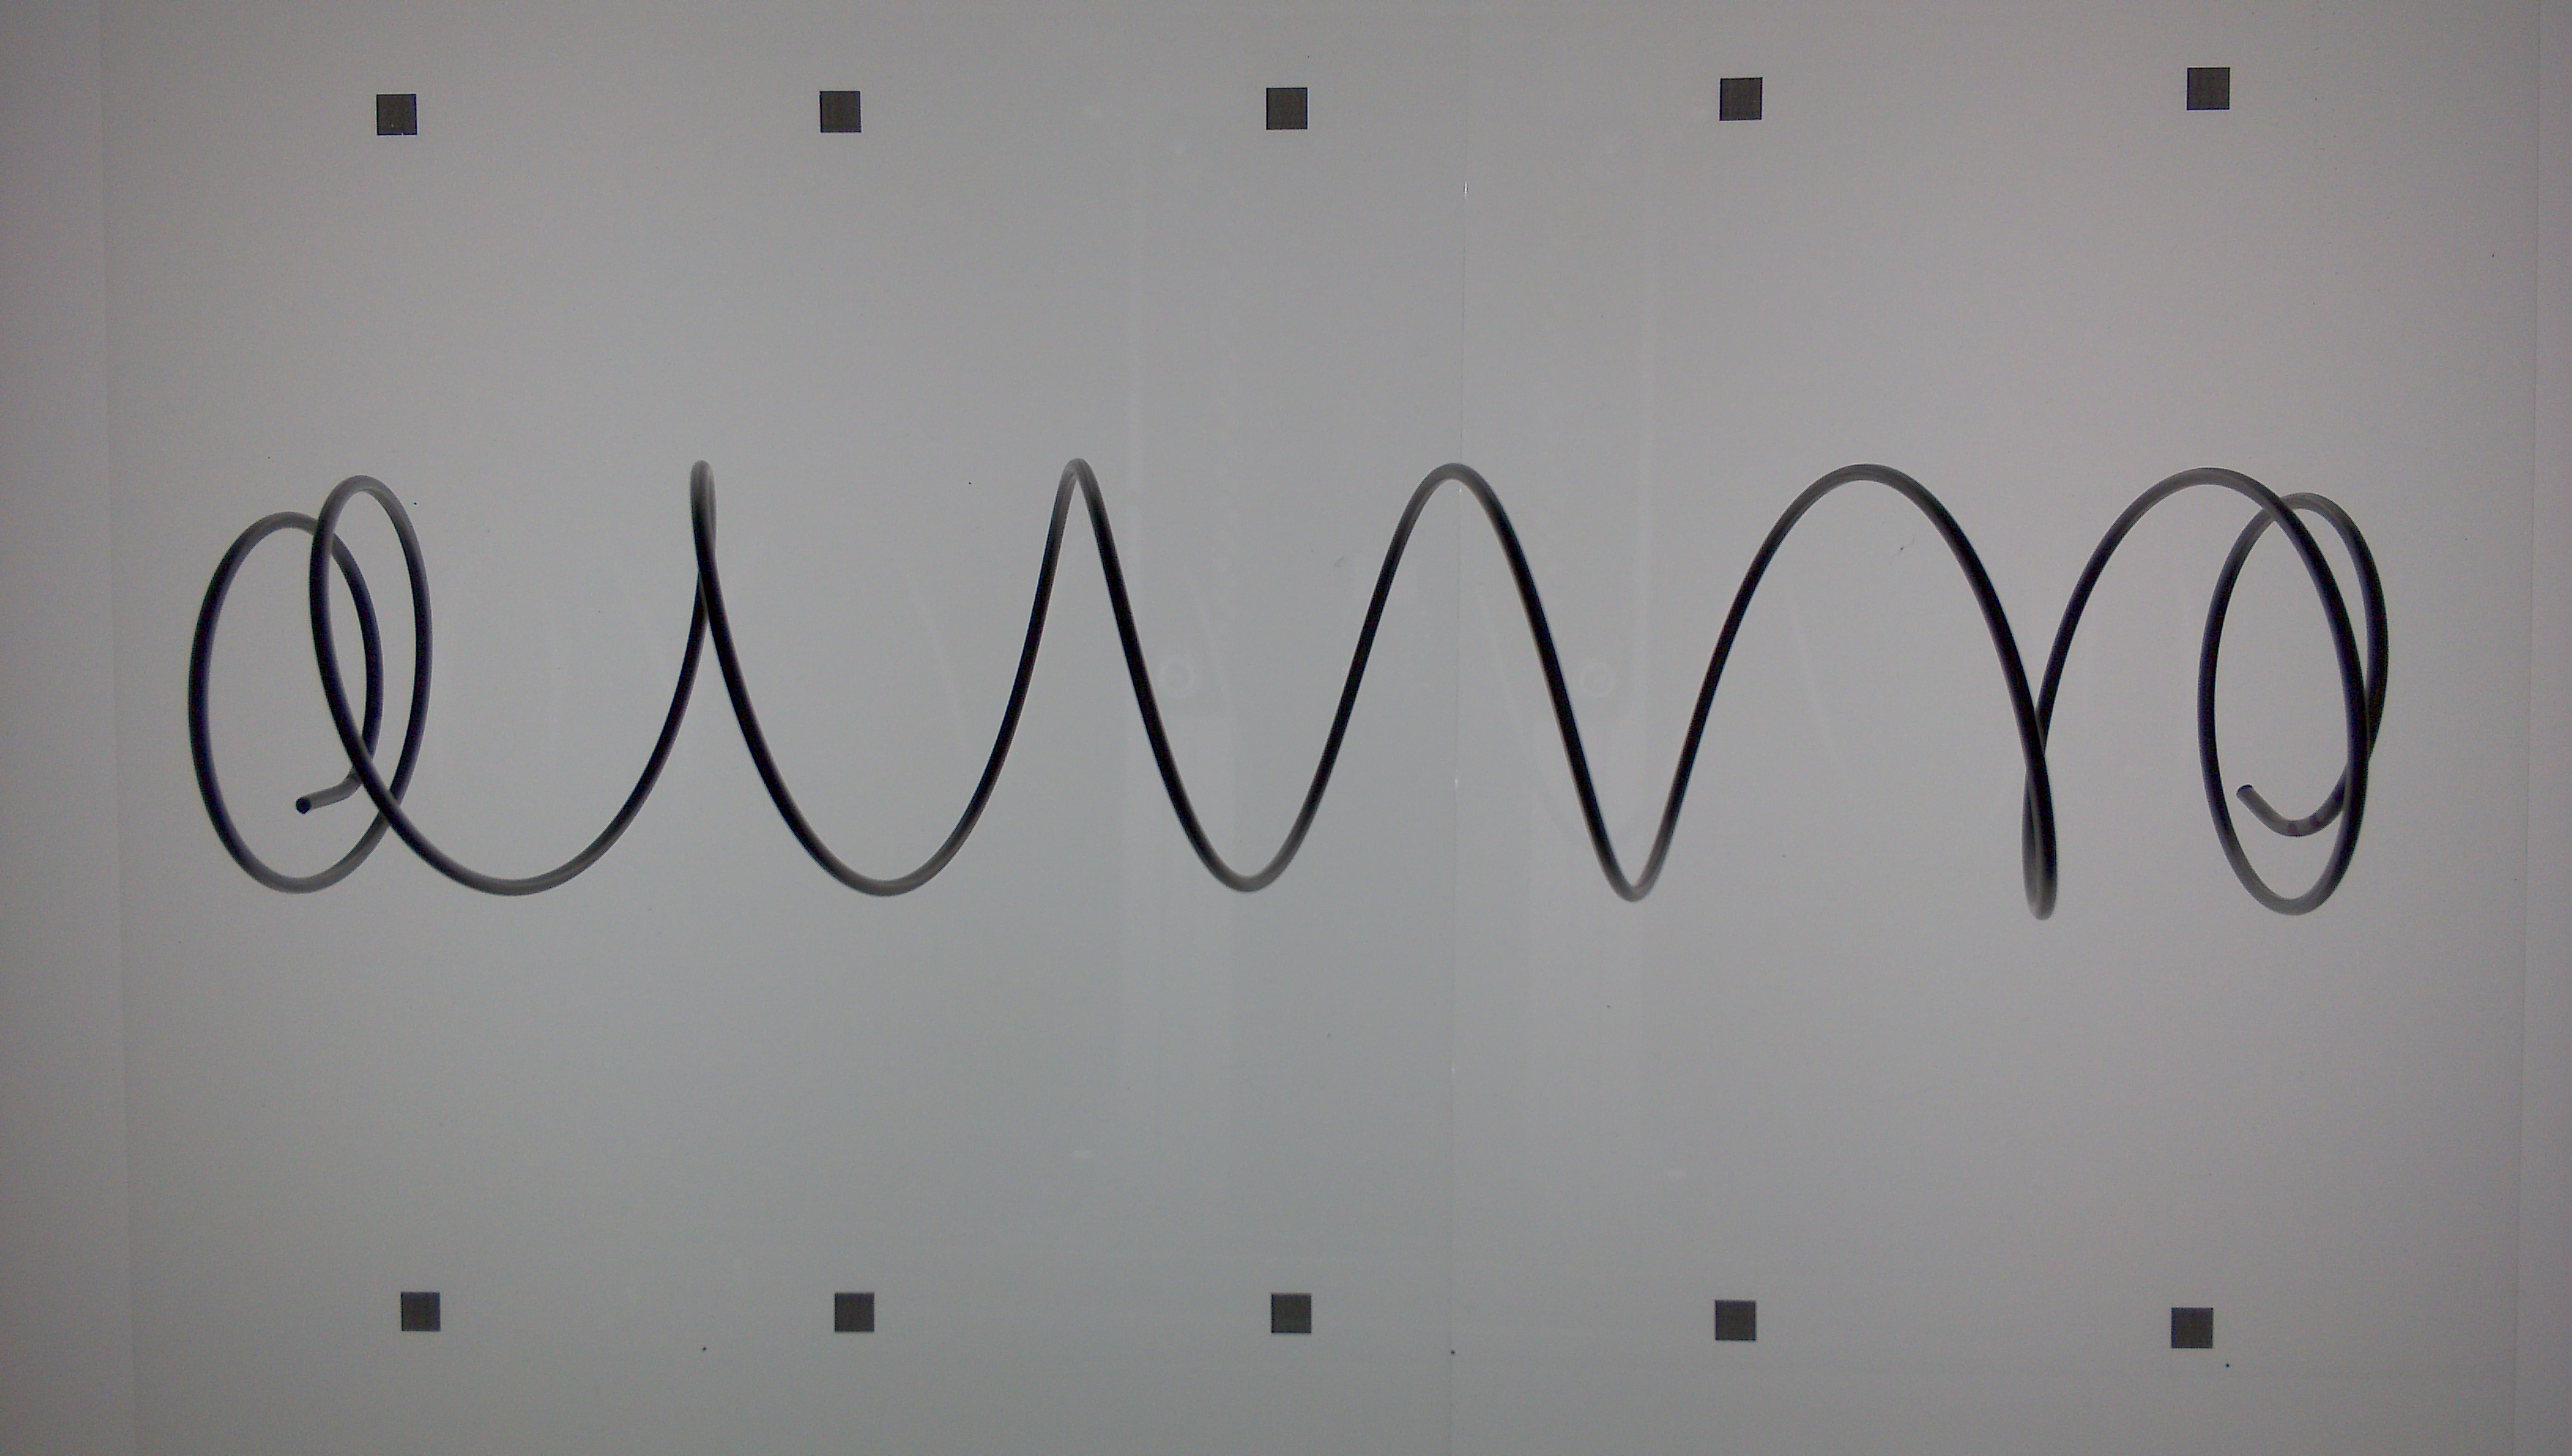
\includegraphics[width=150pt]{bim1.png} at (0,0);

	\node[inner sep=0pt] (russell) at (0,0)
	{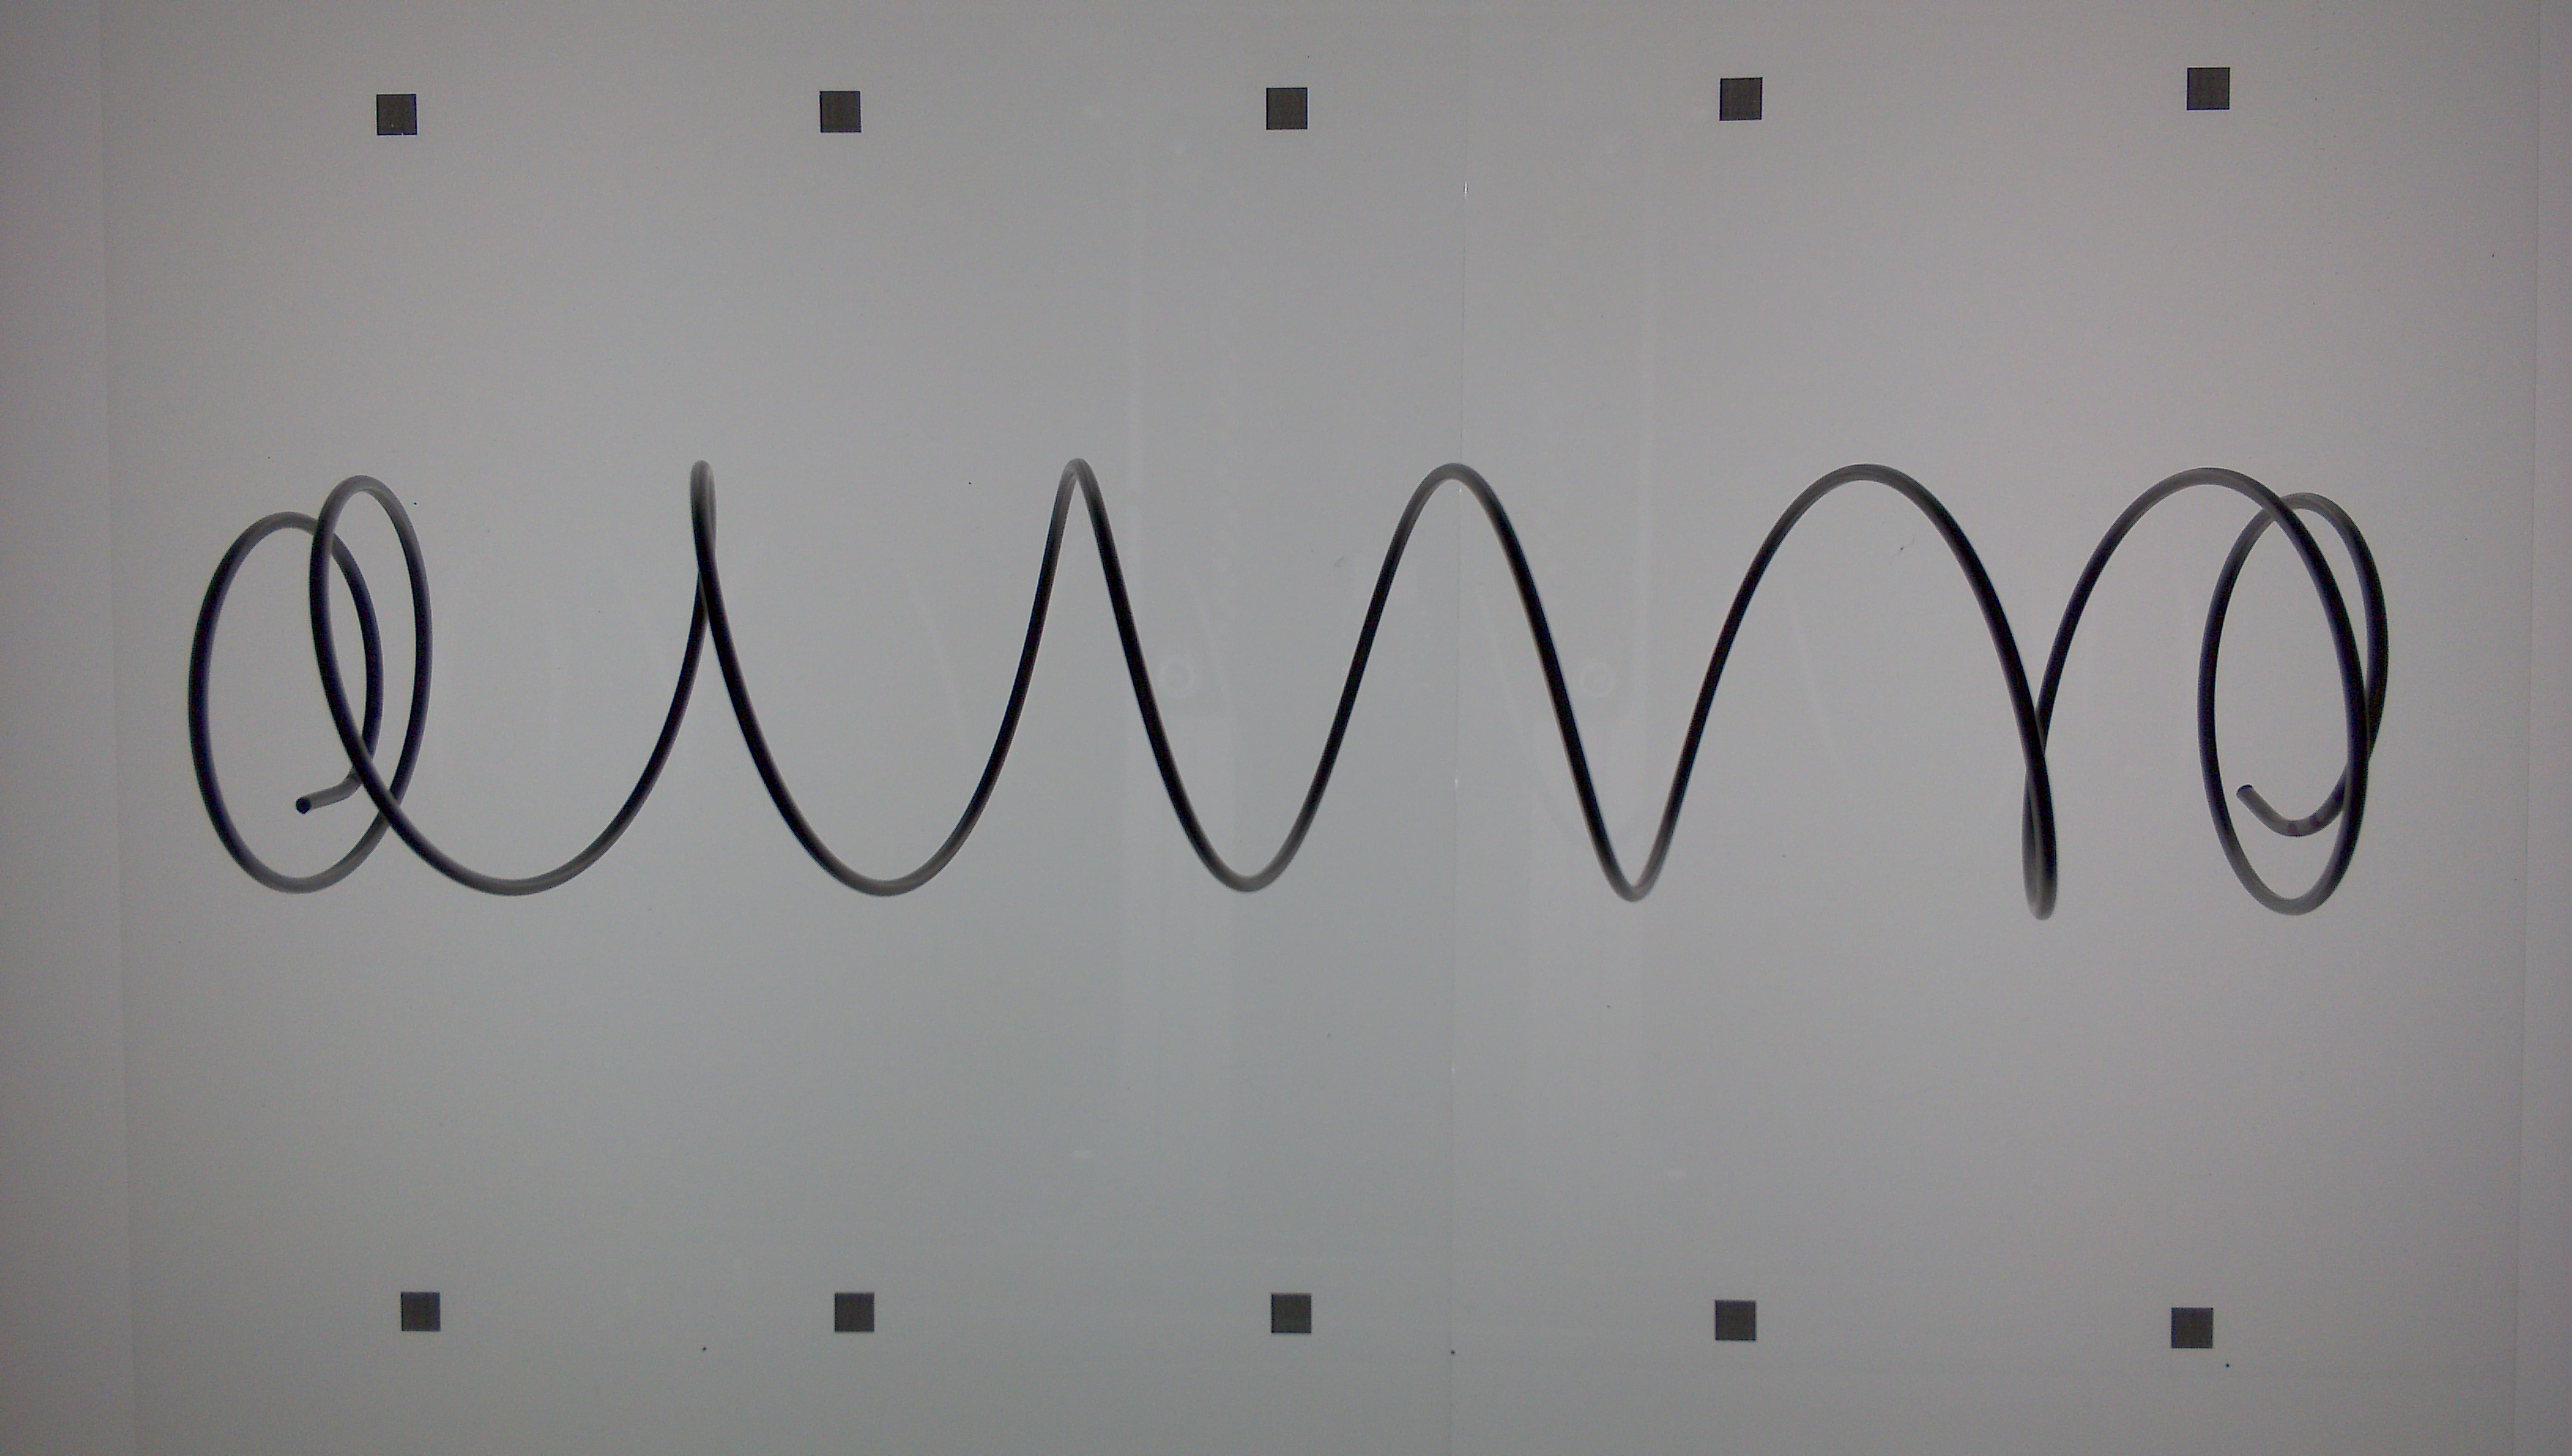
\includegraphics[width=10cm, height=6cm]{bim1.png}};
	\draw[color = blue, thick ] (-5,-1.977)--(5,-1.97);
	\draw[color = blue,thick] (-5,1.97)--(5,1.97);
	\draw[color = black!30!white , dashed, thick] (-4,3)--(-4,-3);
	\draw[color = black!30!white , dashed, thick] (4,3)--(4,-3);
	\draw[color = red, thick] (-4,3)--(-4,2)--(4,2)--(4,3);
	\draw[color = red, thick] (-4,-3)--(-4,-2)--(4,-2)--(4,-3);
	
	\draw[<->,color = black!10!white](-5,1.5)-- node[above]{vec}(-4,1.5);
	\draw[<->,color = black!10!white](5,1.5)-- node[above]{vec}(4,1.5);
	
	\draw[<->,color = black!10!white](-0.5,3)-- node[left]{sep}(-0.5,2);
	\draw[<->,color = black!10!white](-0.5,-3)-- node[left]{sep}(-0.5,-2);
	
	\end{tikzpicture}
\end{document}	